\documentclass[11pt, a4paper]{article}
\usepackage[utf8]{inputenc}
\usepackage[T1]{fontenc}
\usepackage[a4paper, margin=2.5cm]{geometry}
\usepackage[english]{babel}

\usepackage{amsmath}
\usepackage{amssymb}
\usepackage{booktabs}
\usepackage{tabularx}
\usepackage{fancyhdr}
\usepackage{xcolor}
\usepackage{graphicx}
\usepackage{float}
\usepackage{hyperref}

\hypersetup{
    colorlinks=true,
    linkcolor=blue,
    urlcolor=blue,
    pdftitle={Microstates and Macroscopic Thermodynamics of a Binary System}
}

% Page Header and Footer setup
\pagestyle{fancy}
\fancyhf{}
\rhead{\small Statistical Physics Lab 1}
\lhead{\small Microstates of a System of Coins}
\lfoot{\small UC3M}
\rfoot{\small Page \thepage}
\renewcommand{\headrulewidth}{0.4pt}
\renewcommand{\footrulewidth}{0.4pt}

\fancypagestyle{plain}{%
  \fancyhf{}%
  \lfoot{\small UC3M}%
  \rfoot{\small Page \thepage}%
  \renewcommand{\headrulewidth}{0pt}%
  \renewcommand{\footrulewidth}{0.4pt}%
}

% All numerical results are generated by `python main.py`
\input{results}

\newcommand{\kB}{k_{\mathrm{B}}}
% Expandable input for generated table rows (\input is not expandable in a tabular)
\makeatletter\newcommand{\tabinput}[1]{\@@input #1 }\makeatother

\title{\textbf{Microstates and Macroscopic Thermodynamics of a Binary System}\\
\large Statistical Physics --- Laboratory Practice 1}

\author{\input{authors}\\[0.3em]
\small Department of Physics, Universidad Carlos III de Madrid}

\date{\today}

\begin{document}

\maketitle

\begin{abstract}
\noindent We study a system of $N$ independent unbiased coins as an exact model of a two-state assembly. A modular Python package enumerates all $2^N$ microstates by bitwise encoding, computes the multiplicities $\Omega(N,k)$ exactly and in log-space, and evaluates probabilities and Boltzmann entropies. Full enumeration is limited by its $\mathcal{O}(2^N)$ cost: the largest system fully enumerated within five minutes of wall-clock time is $N=\NverifyVal$. For the assigned system of $N=\Nval$ coins the equal-split macrostate has probability $\PhalfHeads$, while $\PtenHeads$ of all outcomes lie within $\pm10$ heads of it. Entropy differences between macrostates are of order $10\,\kB$, i.e.\ $10^{-22}$\,J/K. As $N\to10^{23}$ the relative width of the distribution falls to $\TLwidth$, and macroscopic decreases of entropy become unobservable. This is the statistical content of the Second Law.
\end{abstract}

\vspace{0.5em}
\noindent \textbf{Repository:} \url{https://github.com/olivia614/StatPhys_Lab1_GroupA}

\vspace{1em}

%==========================================================================
\section{Introduction \& Objectives}
%==========================================================================
A microstate of $N$ distinguishable coins is the ordered list of the face of every coin. A macrostate is specified only by the number of heads $k$. Every one of the $2^N$ microstates is equally likely for unbiased coins. The multiplicity of a macrostate is the number of ways to choose which $k$ coins show heads:
\begin{equation}
\Omega(N,k) = \binom{N}{k} = \frac{N!}{k!\,(N-k)!}, \qquad \sum_{k=0}^{N}\Omega(N,k)=(1+1)^N = 2^N .
\label{eq:omega}
\end{equation}
The probability of a macrostate and its Boltzmann entropy are therefore
\begin{equation}
P(N,k) = \frac{\Omega(N,k)}{2^{N}}, \qquad S(N,k) = \kB \ln \Omega(N,k).
\label{eq:PS}
\end{equation}
The objectives are: (i) to enumerate microstates and determine how far brute force can go; (ii) to compute and plot $\Omega(N,k)$ for $N=20$--$100$; (iii) to evaluate probabilities and entropy changes for $N=100+M$; and (iv) to extrapolate to $N\sim10^{23}$ and interpret the Second Law statistically.

%==========================================================================
\section{Methodology \& Collaborative Workflow}
%==========================================================================

\subsection{Environment \& Reproducibility}
The environment is a Conda environment (\texttt{statphys\_lab1}, Python 3.11, NumPy, SciPy, Matplotlib, pytest) specified in \texttt{environment.yml}. Running \texttt{python main.py} regenerates every figure in \texttt{report/figures/} and every number in this report (\texttt{report/results.tex}). The timing study runs with \texttt{python main.py --benchmark}.

\subsection{Version Control \& Repository Architecture}
Development followed a feature-branch workflow on GitHub, with direct pushes to \texttt{main} disabled and pull requests reviewed by at least one teammate. The code is organised as:
\begin{itemize}
    \item \texttt{src/microstates.py}: bitwise enumeration (generator and chunked NumPy versions), benchmark utilities.
    \item \texttt{src/combinatorics.py}: exact big-integer and log-gamma binomial coefficients, floating-point limits.
    \item \texttt{src/thermodynamics.py}: probabilities, entropy, waiting times, Gaussian limit, Monte Carlo tosses.
    \item \texttt{tests/}: 147 \texttt{pytest} tests checking every routine, and the numbers written to this report, against \texttt{math.comb} and exact rational arithmetic (100\% line coverage of \texttt{src/}, 99\% of \texttt{main.py}); the audit is in \texttt{docs/\allowbreak AUDIT.md}.
    \item \texttt{main.py}: orchestrates all calculations; \texttt{report/}: \LaTeX{} source and figures.
\end{itemize}

\subsection{Numerical Uncertainty}
All combinatorial quantities are exact integers or are computed in double precision with relative error below $10^{-12}$; this is verified by unit tests against exact integer arithmetic. They are quoted to three or four significant figures. The only measured quantities are wall-clock times. These are reported as the mean $\pm$ sample standard deviation of three repetitions on a 16-thread laptop CPU.

%==========================================================================
\section{Computational Analysis of Microstates}
%==========================================================================

\subsection{Enumeration for $N=7$}
Each microstate is encoded as an integer $s\in[0,2^N)$ whose bit $i$ is 1 if coin $i$ shows heads and 0 if it shows tails. A Python generator loops over \texttt{range(1 << N)}, producing each microstate once without storing the others, resulting in  $\mathcal{O}(1)$ memory. The macrostate is then the population count of $s$ (\texttt{s.bit\_count()}). For display, we flipped the bits (such as $0000000 \rightarrow 1111111$), thereby swapping heads and tails, so that the listing starts with all heads to match the sample table in the instructions. Table~\ref{tab:macrostate_7} summarizes the $\NsevenTotal$ outcomes for $N=7$, and the complete listing of all possible microstates is given in Appendix~\ref{app:n7}. The counts reproduce row 7 of Pascal's triangle and sum to $2^7$.


\begin{table}[H]
\centering
\caption{Macrostates of $N=7$ coins: multiplicity $\Omega(7,k)$ obtained by enumeration, and probability $P_k$.}
\label{tab:macrostate_7}
\begin{tabular}{cccrc}
\toprule
\textbf{Heads $k$} & \textbf{Tails $7-k$} & \textbf{Example microstate} & $\mathbf{\Omega(7,k)}$ & $\mathbf{P_k}$ \\
\midrule
\tabinput{tables/n7_summary.tex}
\midrule
 & & \textbf{Total} & 128 & 1 \\
\bottomrule
\end{tabular}
\end{table}

\subsection{Maximum Computable $N$ (Full Enumeration):}
Two implementations were timed (Table~\ref{tab:performance}, Fig.~\ref{fig:benchmark}), both on a single core of an Intel Core Ultra 7 258V laptop with 32\,GB of RAM. The first is the pure-Python generator, which loops over every state and increments \texttt{counts[s.bit\_count()]}. The second splits $[0,2^N)$ into blocks of $2^{22}$ consecutive integers and, for each block, counts heads in compiled NumPy code by looking up the popcount of each 16-bit piece of every state in a precomputed table. Both visit every microstate and build the full histogram; no combinatorial shortcut is used. Both reproduce $\Omega(N,k)=\binom{N}{k}$ exactly, which were manually checked.

A least-squares fit of $\log_2 t = a + bN$ to the timed sweeps gives slopes $b=1.013$ (generator) and $b=1.010$ (vectorized), consistent with $b=1$, i.e.\ the time doubles with every added coin. Imposing $t=c\,2^N$, the cost per microstate $c$ (median of $t/2^N$) is $73.0$\,ns for the generator and $19.4$\,ns for the vectorized code, a speedup of $3.8\times$. Extrapolating to $t=300$\,s predicts $N_{\max}\approx31.9$ (generator) and $N_{\max}\approx33.9$ (vectorized).

The prediction was tested with direct runs of the vectorized code (stars in Fig.~\ref{fig:benchmark}). $N=33$ finished in $243.9$\,s and its histogram matched $\Omega(N,k)$ for every $k$, while $N=34$ took $468.4$\,s and exceeds the 5-minute limit. The largest $N$ fully enumerated within five minutes is therefore $N_{\max}=33$. The long runs cost about $28$\,ns per state, more than the $19.4$\,ns of the short sweeps. This is probably due to sustained load on the laptop (thermal or power limiting) and, for $N>32$, to a third 16-bit lookup per state; we did not separate the two effects. Single runs have no error bar. Repeated short timings scatter by up to about 13\% (one standard deviation, Table~\ref{tab:performance}).

\paragraph{Memory.} The generator needs only the $N+1$ counters, measured as a peak of $0.001$\,MB with \texttt{tracemalloc} ($N=20$). The vectorized code works on blocks of $2^{22}$ states and peaked at $168$\,MB ($N=24$), independent of $N$. These figures count only Python/NumPy allocations.

\begin{table}[H]
\centering
\caption{Wall-clock time for building the full histogram of $2^N$ microstates, single core. Entries with ``$\pm$'' are mean $\pm$ sample standard deviation of 3 runs; ``1 run'' entries are single verification runs.}
\label{tab:performance}
\begin{tabular}{cccc}
\toprule
$\mathbf{N}$ & $\mathbf{2^N}$ & \textbf{Generator (s)} & \textbf{Vectorized (s)}  \\
\midrule
\tabinput{tables/benchmark.tex}
\bottomrule
\end{tabular}
\end{table}

\begin{figure}[!htb]
\centering
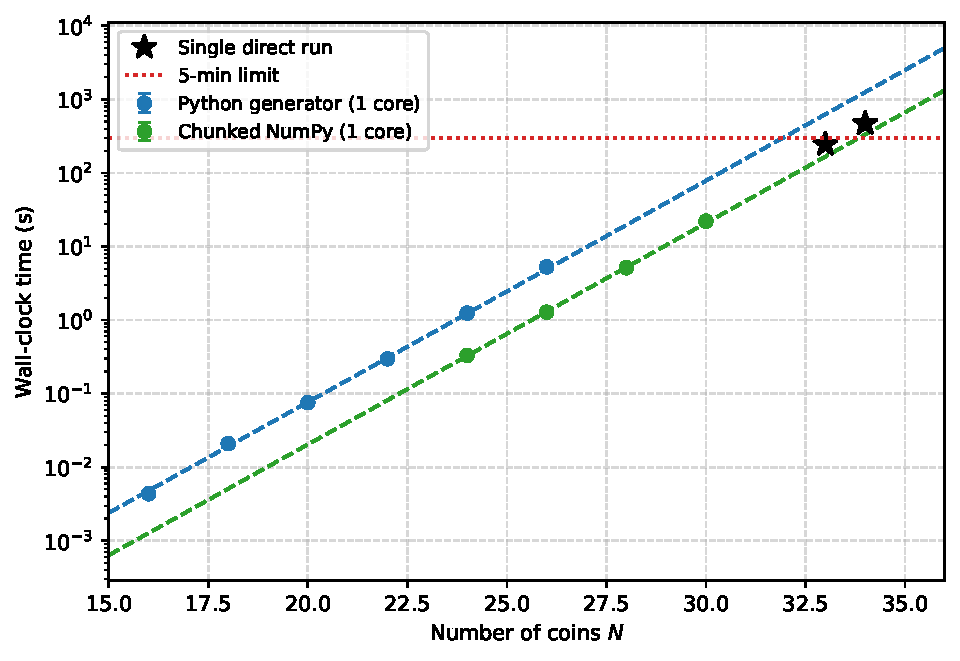
\includegraphics[width=0.62\linewidth]{figures/enumeration_scaling.pdf}
\caption{Enumeration time versus $N$ (log scale). Dashed lines are the exponential fits. The horizontal line is the 5-minute limit.}
\label{fig:benchmark}
\end{figure}

\paragraph{Why larger $N$ cannot be reached.}
The limit is the exponential size of the state space, not the implementation. Each additional coin doubles the number of microstates, and hence the runtime. Even an ideal code at $\sim1$\,ns per state needs $2^{40}$\,ns $\approx18$\,min for $N=40$, and about 36\,years for $N=60$; at our measured $\sim28$\,ns per state, $N=40$ would take about 8.5\,h. Storing the states instead of generating them would need $8\times2^N$ bytes, i.e.\ 8\,GB at $N=30$ and 8\,TB at $N=40$; generators avoid this. Writing the list (as required for $N=7$) costs $N\cdot2^N$ characters, which is already 32\,GB at $N=30$. Fixed-width integer encoding also caps the vectorized method at $N=63$.

\subsection{Macrostate Frequency Calculation}
For these $N$, listing microstates is impossible, so $\Omega(N,k)$ is evaluated directly. Factorials are never formed: the multiplicities and probabilities are computed in log-space with the log-gamma function,
\begin{equation}
\ln \Omega(N,k) = \ln \Gamma(N+1) - \ln \Gamma(k+1) - \ln \Gamma(N-k+1),
\label{eq:lgamma}
\end{equation}
and $P_k=\exp[\ln\Omega(N,k)-N\ln 2]$. These values agree with the exact integers from \texttt{math.comb} to a relative precision of $10^{-12}$ (unit tests). Figure~\ref{fig:distributions} shows the results. The peak multiplicity grows from $\Omega(20,10)=1.848\times10^{5}$ to $\Omega(100,50)=1.009\times10^{29}$, while the peak probability falls from $0.1762$ to $0.0796$. The distribution broadens in $k$ as $\sigma=\sqrt N/2$ (from $2.2$ for $N=20$ to $5.0$ for $N=100$), but it narrows relative to $N$.

\begin{figure}[!htb]
\centering
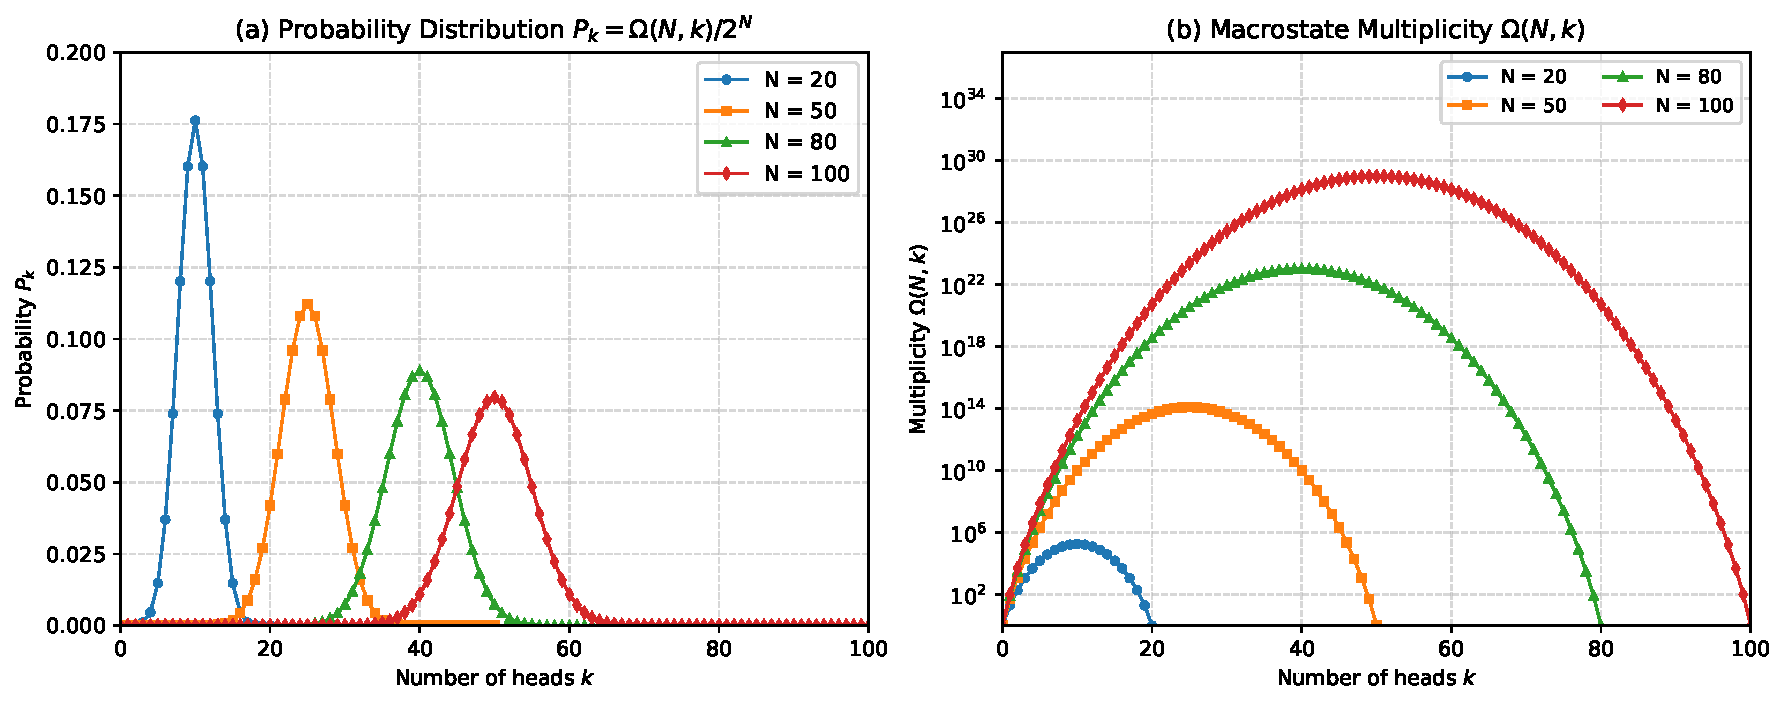
\includegraphics[width=0.92\linewidth]{figures/macrostate_distributions.pdf}
\caption{(a) Normalised probability $P_k=\Omega(N,k)/2^N$. (b) Number of microstates $\Omega(N,k)$ with $k$ heads (log scale), for $N=20$, 50, 80 and 100.}
\label{fig:distributions}
\end{figure}

\subsection{Maximum Computable $N$ (Distribution)}
The distribution needs only $N+1$ numbers, so unlike the enumeration its cost is not exponential in $N$. What limits it is the floating-point representation, and for plotting, the number of points.
\label{sec:distribution-limit}
\begin{itemize}
\item In IEEE double precision, $2^N$ overflows ($>1.80\times10^{308}$) at $N=1024$.
\item A naive $N!/[k!(N-k)!]$ already fails at $N=171$.
\item The central multiplicity $\Omega(N,N/2)\approx 2^N/\sqrt{\pi N/2}$ overflows at $N=1030$. The multiplicity panel of Fig.~\ref{fig:distributions} is computed as $e^{\ln\Omega}$, so it can be drawn only up to this $N$, unless $\ln\Omega$ is plotted instead.
\end{itemize}
Eq.~\eqref{eq:lgamma} never overflows, and $P_k=\exp[\ln\Omega-N\ln2]$ stays finite: the peak is $\sim\sqrt{2/\pi N}$, and the far tails underflow harmlessly to zero. The real limit is rounding: \texttt{gammaln} returns numbers of size $\sim N\ln N$ with relative error $\sim10^{-16}$, so $\ln\Omega$ carries an absolute error $\sim10^{-16}N\ln N$. This is negligible for $\ln\Omega$ itself but not for $\ln P$. We compared $\ln P(N/2)$ with Stirling's result $-\tfrac12\ln(\pi N/2)$, whose own error is $\mathcal{O}(1/N)$. For $N\ge10^{6}$ the difference is dominated by rounding: $2.5\times10^{-7}$ at $N=10^{6}$, $1.8\times10^{-5}$ at $10^{10}$, $1.7\times10^{-3}$ at $10^{12}$ and $1.0\times10^{-2}$ at $10^{13}$. At $N=10^{15}$ the difference is $3.75$, i.e.\ the probability is wrong by a factor $\sim40$, because the spacing of doubles near $\ln\Omega\approx7\times10^{14}$ is $0.125$ and the three terms of Eq.~\eqref{eq:lgamma} cancel almost completely.

Time and memory are not limiting: computing the full distribution takes $0.04$\,s at $N=10^{6}$ and $0.41$\,s at $N=10^{7}$ (arrays of $8(N+1)$ bytes, about $80$\,MB each at $10^{7}$), and the probabilities sum to $1.000000$. The practical maximum is therefore set by accuracy: the distribution can be computed to better than $10^{-4}$ in $\ln P$ up to $N\approx10^{10}$ and is unreliable beyond $N\approx10^{13}$, while plotting every point is sensible only up to $N\sim10^{6}$. Arbitrary-precision integers would remove the overflow, at a cost that grows with the number of digits ($\approx0.3N$). For $N\sim10^{23}$ neither approach works, and the analytic Stirling/Gaussian expressions of the Section~\ref{sec:thermo} are used instead.

\subsection{Thermodynamic Limit ($N\sim10^{23}$)}
\label{sec:thermo}
Stirling's formula, $\ln N! \approx N\ln N - N + \tfrac12\ln(2\pi N)$, applied to Eq.~\eqref{eq:omega} with $k=N/2+\delta$ and expanded to second order in $\delta/N$, gives
\begin{equation}
\ln\Omega(N,k)\simeq N\ln2-\tfrac12\ln\frac{\pi N}{2}-\frac{2\delta^2}{N},
\end{equation}
and hence the de Moivre--Laplace result
\begin{equation}
P(N,k)\simeq\sqrt{\frac{2}{\pi N}}\,\exp\!\left[-\frac{2(k-N/2)^2}{N}\right],\qquad
\mu=\frac N2,\quad\sigma=\frac{\sqrt N}{2},\quad\frac\sigma\mu=\frac1{\sqrt N}.
\label{eq:gauss}
\end{equation}
This is the central limit theorem for $N$ independent two-state elements. At the peak the approximation is already accurate to $0.25\%$ for $N=100$. Figure~\ref{fig:thermo}(a) shows the exact distributions as a function of the fraction $x=k/N$: the peak grows as $\sqrt{N}$ and its width shrinks as $1/\sqrt N$.

For $N=10^{23}$ the absolute width is large, $\sigma=1.58\times10^{11}$ heads, and the most probable single outcome has a tiny probability, $P(N/2)=\sqrt{2/\pi N}=2.52\times10^{-12}$: the system is almost never found at exactly $k=N/2$. The relative width, however, is $\sigma/\mu=3.16\times10^{-12}$ (Fig.~\ref{fig:thermo}(b)), so the fraction of heads is $\tfrac12$ to eleven significant figures.
\begin{itemize}
\item About $99.7\%$ of all outcomes lie within $\pm3\sigma$, i.e.\ $|k/N-\tfrac12|<4.7\times10^{-12}$.
\item A deviation $|k/N-\tfrac12|>10^{-10}$ is a $63\sigma$ event, with probability $\sim3\times10^{-871}$.
\item A $0.1\%$ deviation ($k/N=0.501$) is suppressed relative to the peak by a factor $10^{-8.69\times10^{16}}$.
\end{itemize}
The Gaussian form holds for $|\delta|\ll N^{3/4}$. For macroscopic deviations the exact leading behavior is $\ln\Omega\simeq N\,H(x)$ with $H(x)=-x\ln x-(1-x)\ln(1-x)$, which for $x$ near $\tfrac12$ reduces to $N[\ln2-2(x-\tfrac12)^2]$. The probabilities of such deviations are then $\exp[-\mathcal O(N)]$.

The distribution is therefore effectively a delta function at $k=N/2$: nearly every microstate has the same macroscopic appearance, and the most probable macrostate is the equilibrium state. The number of microstates is $2^N\approx10^{3.0\times10^{22}}$, and the entropy $S=\kB N\ln2\approx0.96$\,J/K is extensive. Entropy differences between macrostates scale as $\Delta S=-2N\kB(x-\tfrac12)^2$, so they are negligible for fixed offsets in $k$ but reach macroscopic values ($\sim10^{-6}$\,J/K at $x=0.501$) for fixed offsets in $x$. The numerical methods of Sec.~\ref{sec:distribution-limit} cannot reach this $N$, so these results are analytic.

\begin{figure}[!htb]
\centering
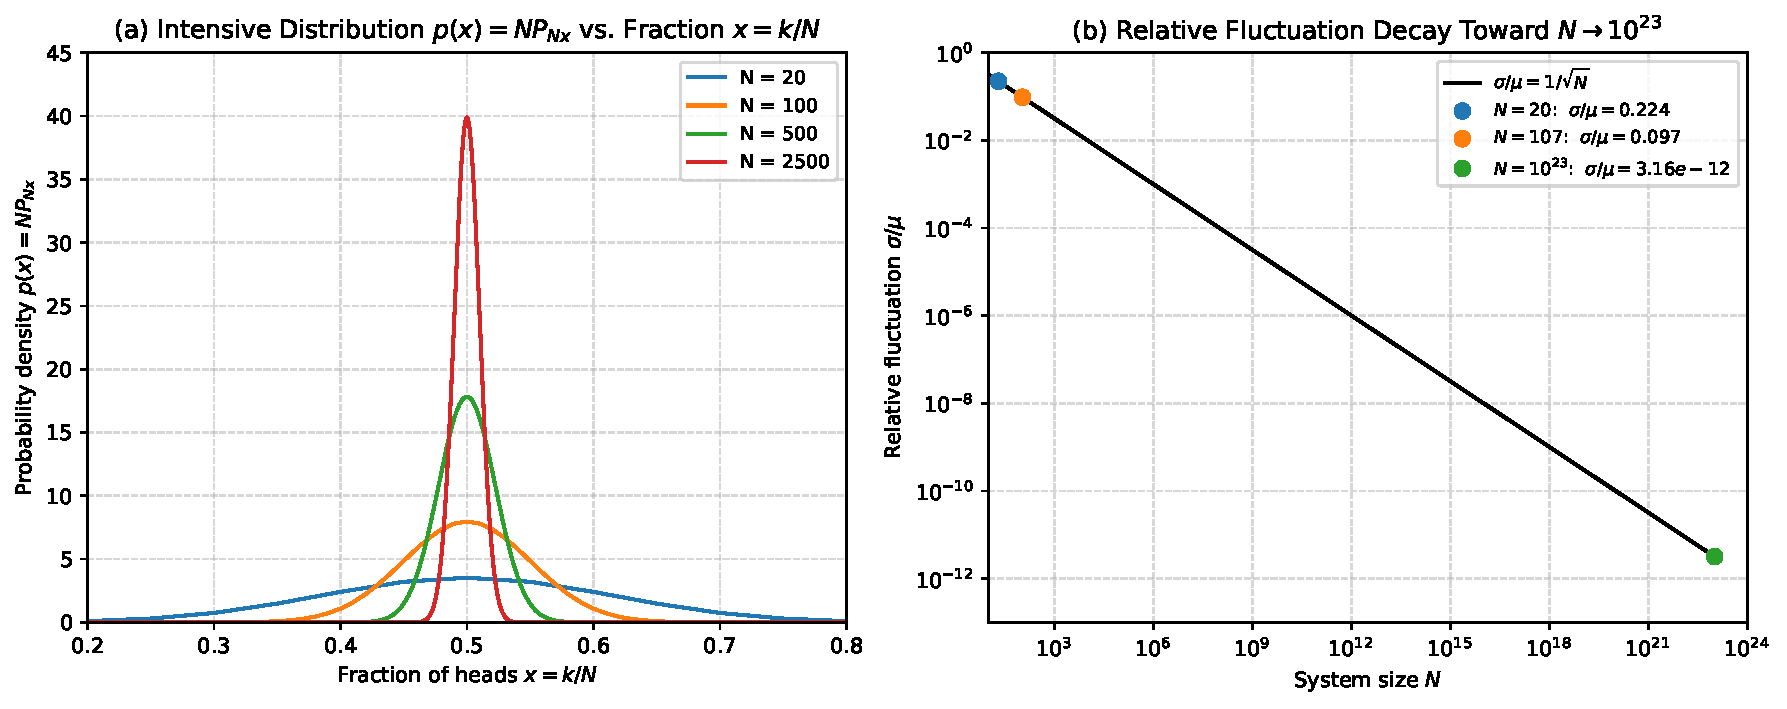
\includegraphics[width=0.92\linewidth]{figures/thermodynamic_limit.pdf}
\caption{(a) Exact intensive distribution $p(x)=N P_{Nx}$ against the fraction $x=k/N$ for $N=20$, 100, 500 and 2500. (b) Relative fluctuation $\sigma/\mu=1/\sqrt N$ from Eq.~\eqref{eq:gauss} (analytic), with the systems used in this report marked.}
\label{fig:thermo}
\end{figure}

%==========================================================================
\section{Probabilities, Entropy, and Thermodynamics}
%==========================================================================

\subsection{Parameter Assignment}
$M$ is the harmonic mean of the last two digits of the team members' NIAs ($\NIAdigits$), $M=n/\sum_i d_i^{-1}=\Mexact$, rounded to $M=\Mval$. Hence $N=100+M=\Nval$ coins, with $2^N=\TotalStates$ microstates. \HalfNote

\subsection{Probability and Entropy Analysis}
All probabilities follow from Eq.~\eqref{eq:PS}. Range probabilities are sums over $k$, evaluated with a log-sum-exp to avoid underflow. The entropy difference between two macrostates is defined as $\Delta S_{k_1k_2}\equiv S(k_1)-S(k_2)$, so that
\begin{equation}
\frac{\Delta S_{k_1k_2}}{\kB}=\ln\frac{\Omega(N,k_1)}{\Omega(N,k_2)},\qquad \kB=1.380649\times10^{-23}\ \mathrm{J/K}.
\end{equation}
$\Delta S_{k_1k_2}$ is positive when $k_1$ is the more disordered macrostate (larger $\Omega$) and negative otherwise. Results are collected in Table~\ref{tab:entropy} and illustrated in Fig.~\ref{fig:prob}.

\begin{table}[H]
\centering
\caption{Probabilities and entropy changes for $N=\Nval$ coins (questions 1--9).}
\label{tab:entropy}
\begin{tabularx}{\linewidth}{@{}lX r@{}}
\toprule
\textbf{Question} & \textbf{Quantity} & \textbf{Result} \\
\midrule
1 & $P(k=30)$, with $\Omega=\OmegaThirty$ & $\PthirtyHeads$ \\
2 & $P(k=\Nhalf)$, with $\Omega=\OmegaHalf$ & $\PhalfHeads$ \\
3 & $P(\Nhalf-10\le k\le\Nhalf+10)$ heads & $\PtenHeads$ \\
4 & $P(\Nhalf-20\le N-k\le\Nhalf+20)$ tails & $\PtwentyTails$ \\
\midrule
5 & $\Delta S_{k_1k_2}$: $k_1=\dSAfrom$, $k_2=\dSAto$ heads & $\dSA\,\kB=\dSASI$ J/K \\
6 & $\Delta S_{k_1k_2}$: $k_1=\dSBfrom$, $k_2=\dSBto$ heads & $\dSB\,\kB=\dSBSI$ J/K \\
7 & $\Delta S_{k_1k_2}$: $k_1=\dSCfrom$, $k_2=\dSCto$ heads & $\dSC\,\kB=\dSCSI$ J/K \\
\midrule
8 & $P(k=8)$; mean wait at 1 toss/s & $\PeightHeads$;\ \ $\WaitEightS$ s \\
9 & $P(\Nhalf)/P(N/2+10=\MPlus)$ & $\RatioPlus$ \\
  & $P(\Nhalf)/P(N/2-10=\MMinus)$ & $\RatioMinus$ \\
\bottomrule
\end{tabularx}
\end{table}

\begin{figure}[!htb]
\centering
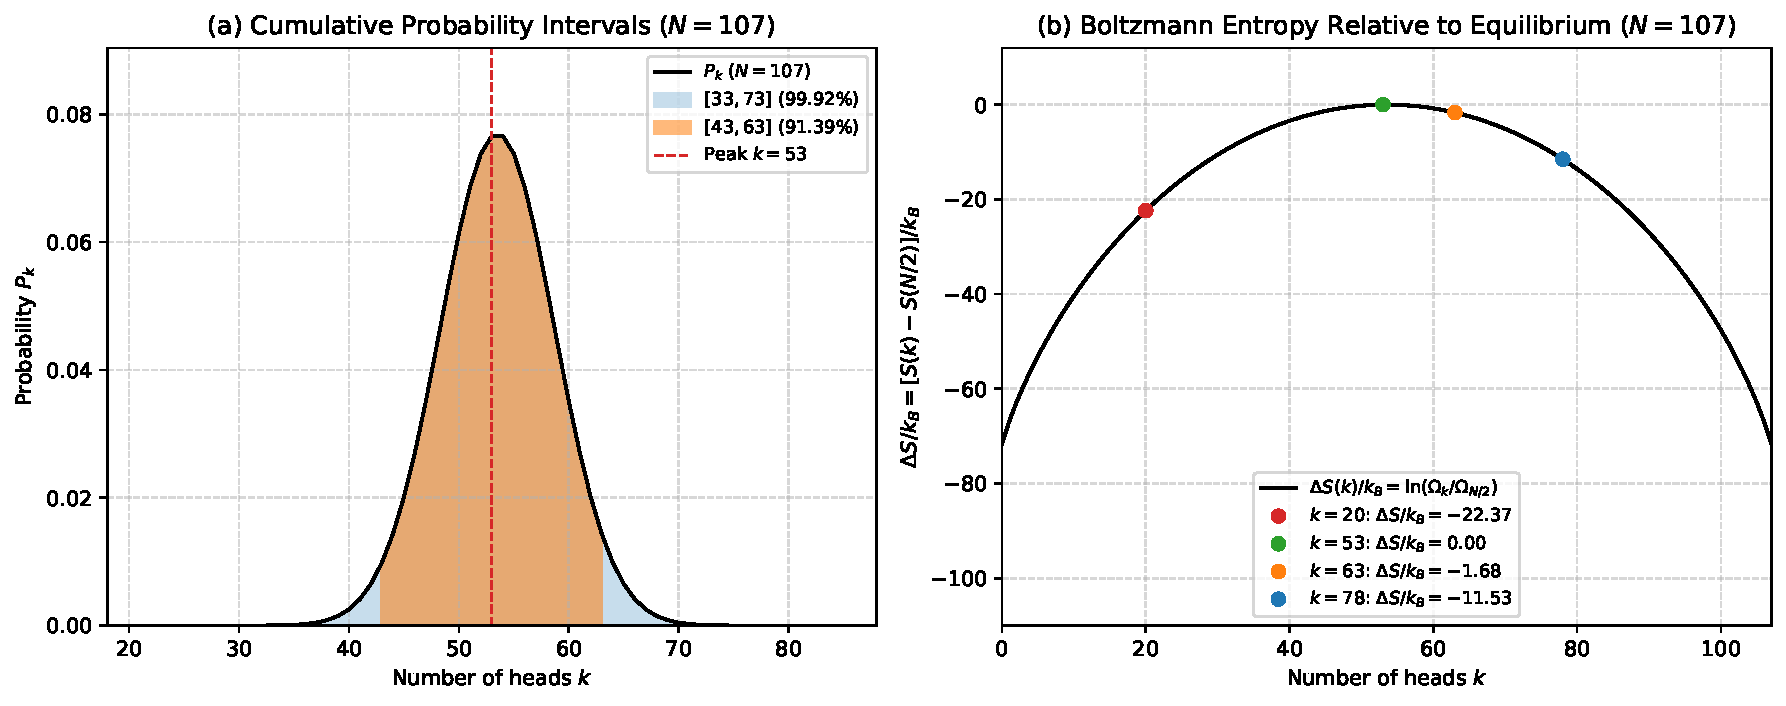
\includegraphics[width=0.92\linewidth]{figures/probabilities_entropy.pdf}
\caption{(a) $P_k$ for $N=\Nval$; the shaded band is $\Nhalf\pm10$ heads and dotted lines mark $k=30$ and $N/2\pm10$. (b) Entropy $S/\kB=\ln\Omega$; points mark the states used in questions 5--8.}
\label{fig:prob}
\end{figure}

\paragraph{Discussion of questions 1--4.}
Although $\Nhalf$ heads is the single most probable outcome, its probability is only $\PhalfHeads$ because there are $\Nval+1$ possible macrostates. Ranges matter more: about $\sigma=\sqrt N/2\approx\SigmaN$, so $\pm10$ heads covers $\approx\TenInSigma\sigma$ and holds $\PtenHeads$ of the probability. The $\pm20$-tails window ($\approx\TwentyInSigma\sigma$) misses only $\PtwentyTailsComp$. By contrast, $k=30$ lies $\ThirtyInSigma\sigma$ below the mean and has probability $\PthirtyHeads$.

\paragraph{Question 8.}
Each toss is an independent trial with success probability $p=P(N,8)$. The number of tosses until the first success is therefore geometric, with mean $1/p$. At one toss per second the expected wait is $\WaitEightS$\,s, which is $\WaitEightYears$ years or $\WaitEightUniverse$ times the age of the Universe.

\paragraph{Question 9.}
The equal split is $\RatioPlus$ times more likely than $N/2+10=\MPlus$ heads, and $\RatioMinus$ times more likely than $N/2-10=\MMinus$ heads.

\subsection{Second Law of Thermodynamics Interpretation (question 10)}
None of these results contradicts the Second Law, because in statistical mechanics the Second Law is a statement about probabilities, not a strict prohibition. The microscopic dynamics (re-tossing coins) are reversible, and every microstate is equally likely, including the ``ordered'' ones. A transition from $k=\Nhalf$ to $k=20$ lowers the entropy by $\Delta S_{k_1k_2}=\dSC\,\kB$ (question 7). It is not forbidden; it is simply $\Omega(\Nhalf)/\Omega(20)=e^{\,\dSCabs}$ times rarer than the reverse. For $N=\Nval$, fluctuations of a few $\kB$ (questions 5--6) do occur: about $\OutsideTenPct\%$ of tosses fall outside $\Nhalf\pm10$. These fluctuations are visible only because $N$ is small. The Second Law is the statement that the macrostate with maximum $\Omega$ (maximum $S$) overwhelmingly dominates, so a spontaneous evolution almost always goes towards higher entropy.

\subsection{The Limit $N\gg1$ (question 11)}
For $N\sim10^{23}$, Eq.~\eqref{eq:gauss} and the log-space routines give:
\begin{itemize}
\item \textbf{Fixed $k$ (30 heads, 8 heads, $N/2\pm10$).} The probability is $\sim2^{-N}$. For example, $P(k=8)=\TLPeight$, so the waiting time and the likelihood ratios of question 9 become $10^{\sim3\times10^{22}}$. These events never happen.
\item \textbf{$P(N/2)$} $=\sqrt{2/\pi N}=\TLPhalf\to0$, and so does any window of fixed width $\pm10$ or $\pm20$: that width is negligible compared with $\sigma=\TLsigma$. What tends to 1 is the probability of any \emph{relative} window $|k/N-\tfrac12|<\varepsilon$.
\item \textbf{Entropy.} Fixed offsets ($N/2+25\to N/2$) give $|\Delta S|\simeq2\delta^2\kB/N\approx10^{-20}\kB\to0$. Macroscopic offsets ($k/N=0.501\to0.5$) give $|\Delta S|=\TLdSkB\,\kB$, i.e.\ about $\TLdSSI$\,J/K, which is a measurable thermodynamic entropy.
\end{itemize}
In the thermodynamic limit, therefore, the probabilistic statement of question 10 becomes a deterministic law. Entropy-decreasing macroscopic fluctuations have probabilities $\exp(-|\Delta S|/\kB)\sim10^{-10^{17}}$, and the Second Law holds without exception in practice.

%==========================================================================
\section{Conclusion}
%==========================================================================
Bitwise enumeration confirms $\Omega(N,k)=\binom Nk$ directly, but the $2^N$ cost limits it to $N=\NverifyVal$ in five minutes, even with vectorization and parallelism. Log-space combinatorics removes the overflow limit and allows exact statements for $N=\Nval$ (it is reliable up to $N\sim10^{10}$), while the asymptotic statements for $N=10^{23}$ use Stirling's formula analytically. The binomial distribution narrows relative to $N$ as $N^{-1/2}$. Entropy-lowering fluctuations, observable for $N\sim10^2$, become unobservable for macroscopic $N$. This is the statistical origin of the Second Law of Thermodynamics.

\appendix
%==========================================================================
\section{AI Collaboration \& Audit Statement}
%==========================================================================
Following Phase~3 of the course guidelines, AI assistance (Anthropic Claude Code, model Claude Opus~5.5) was used for planning, code generation and drafting this report. Every prompt, the files generated and the team's modifications are logged in \texttt{AI\_STATEMENT.md} at the repository root. The planning transcript is in \texttt{docs/ai\_plans/}. Verification consisted of:
\begin{enumerate}
\emergencystretch=3em
\item 147 \texttt{pytest} tests comparing every AI-written routine with exact integer arithmetic (\texttt{math.comb}), identities ($\sum_k\Omega=2^N$, symmetry) and published values ($\Omega(100,50)\approx1.009\times10^{29}$). A later audit added tests of \texttt{main.py} that check each number of Table~\ref{tab:entropy} against exact fractions, and a mutation analysis (11 deliberately injected bugs, 10 detected, 1 equivalent); see \texttt{docs/\allowbreak AUDIT.md}.
\item An independent Monte Carlo cross-check of the distribution ($\chi^2/\text{dof}=\MCchi/\MCdof$).
\item Re-derivation by the team of all formulas in Sections~3--4.
\end{enumerate}
Issues found during the audit are documented in \texttt{AI\_STATEMENT.md}: a floating-point edge case in the overflow-limit routine, and a LAPACK/MKL crash in the Conda environment.


%==========================================================================
\section{Complete list of microstates for $N=7$}
\label{app:n7}
%==========================================================================
\begin{center}
\small
\begin{tabularx}{\linewidth}{@{}l>{\raggedright\arraybackslash}X@{}}
\toprule
\textbf{Macrostate ($\Omega$)} & \textbf{Microstates} \\
\midrule
\tabinput{tables/n7_full.tex}
\bottomrule
\end{tabularx}
\end{center}

%==========================================================================
\section{Core algorithms}
%==========================================================================
\begin{verbatim}
def iter_microstates(n):              # src/microstates.py
    state, total = 0, 1 << n          # 2**n microstates, O(1) memory
    while state < total:
        yield state
        state += 1

counts[state.bit_count()] += 1        # macrostate = number of set bits

# chunked version: popcount a block of 2**22 states in compiled code
states = offsets + np.uint64(block << chunk_bits)
counts += np.bincount(np.bitwise_count(states), minlength=n + 1)

def log_binom(n, k):                  # src/combinatorics.py, Eq. (3)
    return gammaln(n + 1) - gammaln(k + 1) - gammaln(n - k + 1)
\end{verbatim}

\end{document}
